\chapter{スキャンマッチング}
\label{sec:scan_matching}

\section{スキャンマッチングの概要}

スキャンマッチングとは,2つの点群を正しく照合できるような剛体変換$T = \left( R \mid {\bf t} \right) \in \rm{SE}(3)$を求める処理のことです.
今,点群$\mathcal{P} = ({\bf p}_{1}, ..., {\bf p}_{N})$と$\mathcal{Q} = ({\bf q}_{1}, ..., {\bf q}_{M})$を照合させることを考えます.
ただし${\bf p}, {\bf q} \in \mathbb{R}^{3}$です.
このとき,以下のコスト関数を考えます\footnote{実装では式(\ref{eq:huber_loss})に示すフーバー損失を考えますが,本章では説明が煩雑になることを防ぐためにフーバー損失は無視します}.
%
\begin{align}
  E({\bf t}, R) = \sum_{i=1}^{N} \left\| {\bf q}_{i} - \left( R {\bf p}_{i} + {\bf t} \right) \right\|_{2}^{2}
  \label{eq:icp_cost_SO(3)}
\end{align}
%
ここで${\bf q}_{i}$は,${\bf p}_{i}$を剛体変換した点$R {\bf p}_{i} + {\bf t}$に最も近い$\mathcal{Q}$内の点です.
なお,このような最も近い点である最近傍点を探索するためにはkd木などを用いますが,本書で示す実装では{\it nanoflann}\footnote{ \url{https://github.com/jlblancoc/nanoflann} }というライブラリを利用します.

式(\ref{eq:icp_cost_SO(3)})は,以下のように書くことも可能です.
%
\begin{align}
  E(T) = \sum_{i=1}^{N} \left\| {\bf q}_{i} - T {\bf p}_{i} \right\|_{2}^{2}
  \label{eq:icp_cost_SE(3)}
\end{align}
%
なお式(\ref{eq:icp_cost_SE(3)})の形式で記述する場合,${\bf p}, {\bf q} \in \mathbb{R}^{4}$となり,それぞれの4要素目には1が入ることになります.
そのため,$T {\bf p}$も4要素目が1の4次元ベクトルになりますが,${\bf q}$の4要素目も1となるため,${\bf q} - T {\bf p}$の4要素目は常に0になります.
そのため,結果としてコスト関数の値は式(\ref{eq:icp_cost_SO(3)})に示す値と同じになります.
なお以下では,${\bf q} - T {\bf p}$を残差ベクトル${\bf r}$として定めます.

スキャンマッチングでは,以下に示す剛体変換を求めることを考えます.
%
\begin{align}
  T^{*} = \argmin_{T} E(T)
  \label{eq:icp_scan_matching}
\end{align}
%
式(\ref{eq:icp_scan_matching})は,コスト関数$E$を最小化する姿勢$T^{*}$を求めるという意味になります.
この$T^{*}$は,一般的に反復処理を行うことで求めるられるため,{\bf Iterative Closest Points}(ICP)スキャンマッチングとも呼ばれます.
なお式(\ref{eq:icp_cost_SE(3)})に示すコストを最小にするスキャンマッチングは,対応する点同士の距離を最小にするため,point-to-point ICPとも呼ばれます.

point-to-point ICPは一般的にノイズに脆弱であるといわれています.
そのため本書では,より頑健性の高い点と面の距離を最小化するpoint-to-plane ICPについて考えます.
point-to-plane ICPでは,以下のコスト関数を考えます.
%
\begin{align}
  E(T) = \sum_{i=1}^{N} \left( {\bf n}_{i}^{\top} {\bf r}_{i} \right)^{2}
  \label{eq:point-to-plane_icp_cost_SE(3)}
\end{align}
%
ここで${\bf n}_{i}$は,${\bf q}_{i}$の周辺の点を用いて計算した面の3次元空間内での法線ベクトルであり,$r = {\bf n}_{i}^{\top} {\bf r}_{i}$を残差として考えます.
図\ref{fig:normal_residual}にこれらの関係をまとめます.
なお,${\bf r}$が4次元ベクトルであるため${\bf n}$も4次元ベクトルとなりますが,${\bf r}$の4要素目は常に0であるため,${\bf n}$の4要素目がいくつであっても計算に違いは表れません.

\begin{figure}[!t]
  \centering
  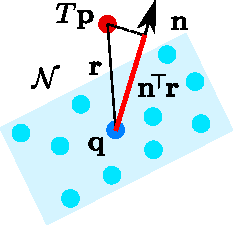
\includegraphics[width=0.2\textwidth]{../figs/normal_residual.pdf}
  \caption{Residual error used in point-to-plane ICP.}
  \label{fig:normal_residual}
\end{figure}

以下ではまず,法線ベクトルの計算方法を述べた後に,残差ベクトルに関するヤコビアンを導出し,このヤコビアンを用いてガウス・ニュートン法により最適化を行う流れについて解説していきます.










\section{法線ベクトルの計算}

ある点${\bf q}$に対する法線ベクトルを計算するにあたり,まず${\bf q}$周辺の点を取得し,この集合を$\mathcal{N}$とします.
そしてこれを用いて,まず平均$\bar{ {\bf q} }$を計算します.
%
\begin{align}
  \bar{ {\bf q} } = \frac{1}{ | \mathcal{N} | } \sum_{ {\bf q}_{i} \in \mathcal{N} } {\bf q}_{i}
  \label{eq:points_mean}
\end{align}
%
次に$\mathcal{N}$の共分散行列$C$を求めます.
%
\begin{align}
  C = \frac{1}{ | \mathcal{N} | } \sum_{ {\bf q}_{i} \in \mathcal{N} } \left( {\bf q}_{i} - \bar{ {\bf q} } \right) \left( {\bf q}_{i} - \bar{ {\bf q} } \right)^{\top}
  \label{eq:points_covariance}
\end{align}
%
そして$C$を固有分解します.
%
\begin{align}
  C = V \Lambda V^{\top}
\end{align}
%
ここで$V = \left( {\bf v}_{1} ~ {\bf v}_{2} ~ {\bf v}_{3} \right)$,$\Lambda = {\rm diag} \left( \lambda_{1}, \lambda_{2}, \lambda_{3} \right)$であり,${\bf v}_{i}$と$\lambda_{i}$は固有ベクトルとそれに対応する固有値になります.


固有値は,各方向における点のばらつきを表す量であり,最小の固有値に対応する固有ベクトルは,点群が最もばらついていない方向,すなわち最も潰れている方向を表します.
そのため,この最小固有値$\lambda_{\min}$が十分に小さい場合,対応する固有ベクトル${\bf v}_{\min}$は,点群が存在する局所平面の法線ベクトルとしてみなすことができます.
このようにして得られた${\bf v}_{\min}$を,点${\bf q}$における法線ベクトル${\bf n}$として定義します.
なお,$\lambda_{\min}$に対して閾値を設定することで,平面性が不十分な点を除外することも可能です.










\section{ヤコビアンの計算}
\label{subsec:point_to_plane_jacobian}

point-to-planeのICPをガウス・ニュートン法を用いて解くにあたり,残差$r = {\bf n}^{\top} {\bf r}$の姿勢$T$に関するヤコビアンを求めます.
このヤコビアンは,連鎖則を用いて以下のように計算できます.
%
\begin{align}
  \frac{ \partial r }{ \partial T } = \frac{ \partial r }{ \partial {\bf r} }
                                      \frac{ \partial {\bf r} }{ \partial T }
\end{align}
%
ここで,$r = {\bf n}^{\top} {\bf r}$であるため,$\partial r / \partial {\bf r}$は明らかに${\bf n}^{\top}$です.
そのため以下では,$\partial {\bf r} / \partial T$についてのみ詳細の計算方法を示します.

残差ベクトル${\bf r}$は,明らかに姿勢$T$に関する関数になっています.
そのため,次式を考えることでヤコビアン$J$を導出します.
%
\begin{align}
  {\bf r} \left( \exp \left( \delta \boldsymbol \xi^{\wedge} \right) T \right) - {\bf r} \left( T \right) =
  J \delta \boldsymbol \xi
  \label{eq:point_plane_icp_jacob_approx}
\end{align}
%
なお$\delta \boldsymbol \xi^{\wedge} = \left( \delta {\bf v}^{\top} ~ \delta \boldsymbol \phi^{\top} \right)^{\wedge} \in \mathfrak{se}(3)$であり,$\exp \left( \delta \boldsymbol \xi^{\wedge} \right) T$は${\rm SE}(3)$の空間で$T$を左から微小摂動させた状態となります.
式(\ref{eq:point_plane_icp_jacob_approx})の左辺を展開していくと以下が得られます.
%
\begin{align}
  \begin{split}
    {\bf q} - \exp \left( \delta \boldsymbol \xi^{\wedge} \right) T {\bf p} - \left( {\bf q} - T {\bf p} \right)
    %
    = & - \left( \exp \left( \delta \boldsymbol \xi^{\wedge} \right) - I_{4} \right) T {\bf p} \\
    %
    = & - \left( \left( \begin{matrix} I_{3} + \delta \boldsymbol \phi^{\wedge} & \delta {\bf v} \\ {\bf 0}^{\top} & 1 \end{matrix} \right) - I_{4} \right) \left( \begin{matrix} R {\bf p} + {\bf t} \\ 1 \end{matrix} \right) \\
    %
    = & - \left( \begin{matrix} \delta \boldsymbol \phi^{\wedge} & \delta {\bf v} \\ {\bf 0}^{\top} & 0 \end{matrix} \right) \left( \begin{matrix} {\bf p}^{'} \\ 1 \end{matrix} \right) \\
    %
     = & - \left( \begin{matrix} \delta \boldsymbol \phi^{\wedge} {\bf p}^{'} + \delta {\bf v} \\ 0 \end{matrix} \right) \\
    %
     = & \left( \begin{matrix} \left( {\bf p}^{'} \right)^{\wedge} \delta \boldsymbol \phi - \delta {\bf v} \\ 0 \end{matrix} \right) \\
     %
     = & \left( \begin{matrix} -I_{3} & \left( {\bf p}^{'} \right)^{\wedge} \\ {\bf 0}^{\top} & {\bf 0}^{\top} \end{matrix} \right) \delta \boldsymbol \xi
  \end{split}
\end{align}
%
なお${\bf p}^{'} = R {\bf p} + {\bf t}$と置き,$\delta \boldsymbol \phi^{\wedge} {\bf p}^{'} = -\left( {\bf p}^{'} \right)^{\wedge} \delta \boldsymbol \phi$を用いました.
よって,残差に対するヤコビアンは以下となります.
%
\begin{align}
  \begin{split}
    \frac{ \partial r }{ \partial T } = & {\bf n}^{\top} \left( \begin{matrix} -I_{3} & \left( {\bf p}^{'} \right)^{\wedge} \\ {\bf 0}^{\top} & {\bf 0}^{\top} \end{matrix} \right) \\
    %
    = & \left( \begin{matrix} -{\bf n}^{\top} & {\bf n}^{\top} \left( {\bf p}^{'} \right)^{\wedge} \end{matrix} \right) \in \mathbb{R}^{1 \times 6}
  \end{split}
  \label{eq:point_to_plane_icp_jacobian}
\end{align}
%
ただし最後の${\bf n} \in \mathbb{R}^{3}$は3次元の法線ベクトルになります.













\section{ガウス・ニュートン法を用いた最適化}

式(\ref{eq:point_to_plane_icp_jacobian})に示すヤコビアンを用いて,point-to-planeのICPスキャンマッチングをガウス・ニュートン法で解くにあたり,ヘッセ行列と勾配ベクトルを以下のように求めます.
%
\begin{align}
  \begin{gathered}
    H = \sum_{i=1}^{N} J_{i}^{\top} J_{i} \\
    {\bf b} = \sum_{i=1}^{N} J_{i}^{\top} r_{i} 
  \end{gathered}
  \label{eq:point_to_plane_icp_hessian_and_gradient}
\end{align}
%
ただしフーバー損失を用いる場合は,式(\ref{eq:huber_loss_prime})を用いて$w_{i} = \rho^{\prime} \left( r_{i}^{2} \right)$を定め,$H = \sum_{i} w_{i} J_{i}^{\top} J_{i}$,${\bf b} = \sum_{i} w_{i} J_{i}^{\top} r_{i}$を計算します.
そして,式(\ref{eq:point_to_plane_icp_hessian_and_gradient})に示す$H$と${\bf b}$を用いて,$H \delta \boldsymbol \xi = -{\bf b}$を満たす$\delta \boldsymbol \xi$を求めます.
最後に,以下のように状態を更新します.
%
\begin{align}
  T \leftarrow \exp \left( \delta \boldsymbol \xi^{\wedge} \right) T
\end{align}
%
この更新を,$\| \delta \boldsymbol \xi \|_{2} \leq \epsilon$,もしくは規定回数繰り返すまで実行することで,式(\ref{eq:icp_scan_matching})に示す$T^{*}$が得られたとみなします.
なお$\epsilon$は任意の定数です.












\section{実用にあたって}
\label{sec:scan_matching_実用にあたって}

スキャンマッチングを正確に実行するためには,いかに良い初期値を得るかが極めて重要になります.
初期値の精度が高ければ,対応点探索は安定して動作し,スキャンマッチングは高い精度で最適解に収束します.
一方で初期値の誤差が大きくなると対応点探索に失敗しやすくなり,スキャンマッチングはうまく機能しなくなります.
なお,スキャンマッチングを実行した結果,コスト関数を最小にしない解に収束してしまうこともありますが,このような解は{\bf 局所最適解}(Local Minima)と呼ばれます.

このような誤対応の影響を軽減するために,ロバストカーネルであるフーバー損失を導入することが有効です.
フーバー損失は,大きな残差の影響を抑えることで,誤対応による最適化の劣化をある程度防ぐことができます.
しかし,フーバー損失の導入は万能ではありません.
例えば,多数の誤対応の中に少数の正しい対応が含まれている場合でも,それらの残差が大きければ,フーバー損失により重みが下がり,正しい対応の影響までもが過小評価されてしまうことがあります.
その結果,フーバー損失を使わない場合にスキャンマッチングが成功し,逆に導入したことで失敗するケースもあり得ます.
したがって,フーバー損失のパラメータ $\delta$ は慎重に調整する必要があります.
それでも一般的には,フーバー損失を導入することでスキャンマッチングのロバスト性は向上します.

なお,スキャンマッチング単体では良好な初期値を毎フレーム安定して得ることは困難です.
特に移動速度や回転速度が大きい場合,その影響は顕著になります.
このような問題を補うためには,IMUなどの外部センサと併用して,より正確な初期位置を与えることが効果的です.
次章では,LiDARとIMUをルーズカップリングにより統合する手法について解説します.

また初期値だけでなく,スキャンマッチングを行う環境にも注意しなければなりません.
スキャンマッチングは基本的に,幾何的な拘束を基に剛体変換を求めるため,正しい解が得られるためには良い拘束が得られる環境である必要があります.
もし適切な拘束が得られない場合にガウス・ニュートン法を解くと,$H \delta \boldsymbol \xi = -{\bf b}$を満たす$\delta \boldsymbol \xi$を適切に求められなくなります.
これは$H$が正則でなくなり,この逆行列が定まらなくなるためです.
このような例は{\bf 縮退}(Degeneracy)したケースと呼ばれ,スキャンマッチングがそもそも機能しないケースとなります.
なお縮退を検出する方法として,式(\ref{eq:point_to_plane_icp_hessian_and_gradient})に示すヘッセ行列の固有値分解を行い,その最小固有値を確認する方法もあります.
ヘッセ行列の最小固有値が極端に小さい場合,行列がランク落ちして正しい逆行列が求められなくなり,結果として最適化が破綻することになります.

